%%%%%%%%%%%%%%%%%%%%%%%%%%%%%%%%%%%%%%%%%
% baposter Portrait Poster
% LaTeX Template
% Version 1.0 (15/5/13)
%
% Created by:
% Brian Amberg (baposter@brian-amberg.de)
%
% This template has been downloaded from:
% http://www.LaTeXTemplates.com
%
% License:
% CC BY-NC-SA 3.0 (http://creativecommons.org/licenses/by-nc-sa/3.0/)
%
%%%%%%%%%%%%%%%%%%%%%%%%%%%%%%%%%%%%%%%%%

%----------------------------------------------------------------------------------------
%	PACKAGES AND OTHER DOCUMENT CONFIGURATIONS
%----------------------------------------------------------------------------------------

\documentclass[a0paper,portrait]{baposter}

\usepackage[font=small,labelfont=bf]{caption} % Required for specifying captions to tables and figures
\usepackage{booktabs} % Horizontal rules in tables
\usepackage{relsize} % Used for making text smaller in some places
\usepackage[utf8]{inputenc}
\usepackage{amsmath}
\usepackage{amsfonts}
\usepackage{amssymb}
\graphicspath{{figures/}} % Directory in which figures are stored

\definecolor{bordercol}{RGB}{40,40,40} % Border color of content boxes
\definecolor{headercol1}{RGB}{186,215,230} % Background color for the header in the content boxes (left side)
\definecolor{headercol2}{RGB}{80,80,80} % Background color for the header in the content boxes (right side)
\definecolor{headerfontcol}{RGB}{0,0,0} % Text color for the header text in the content boxes
\definecolor{boxcolor}{RGB}{186,215,230} % Background color for the content in the content boxes

\begin{document}



\background{ % Set the background to an image (background.pdf)
\begin{tikzpicture}[remember picture,overlay]
\draw (current page.north west)+(-2em,2em) node[anchor=north west]
{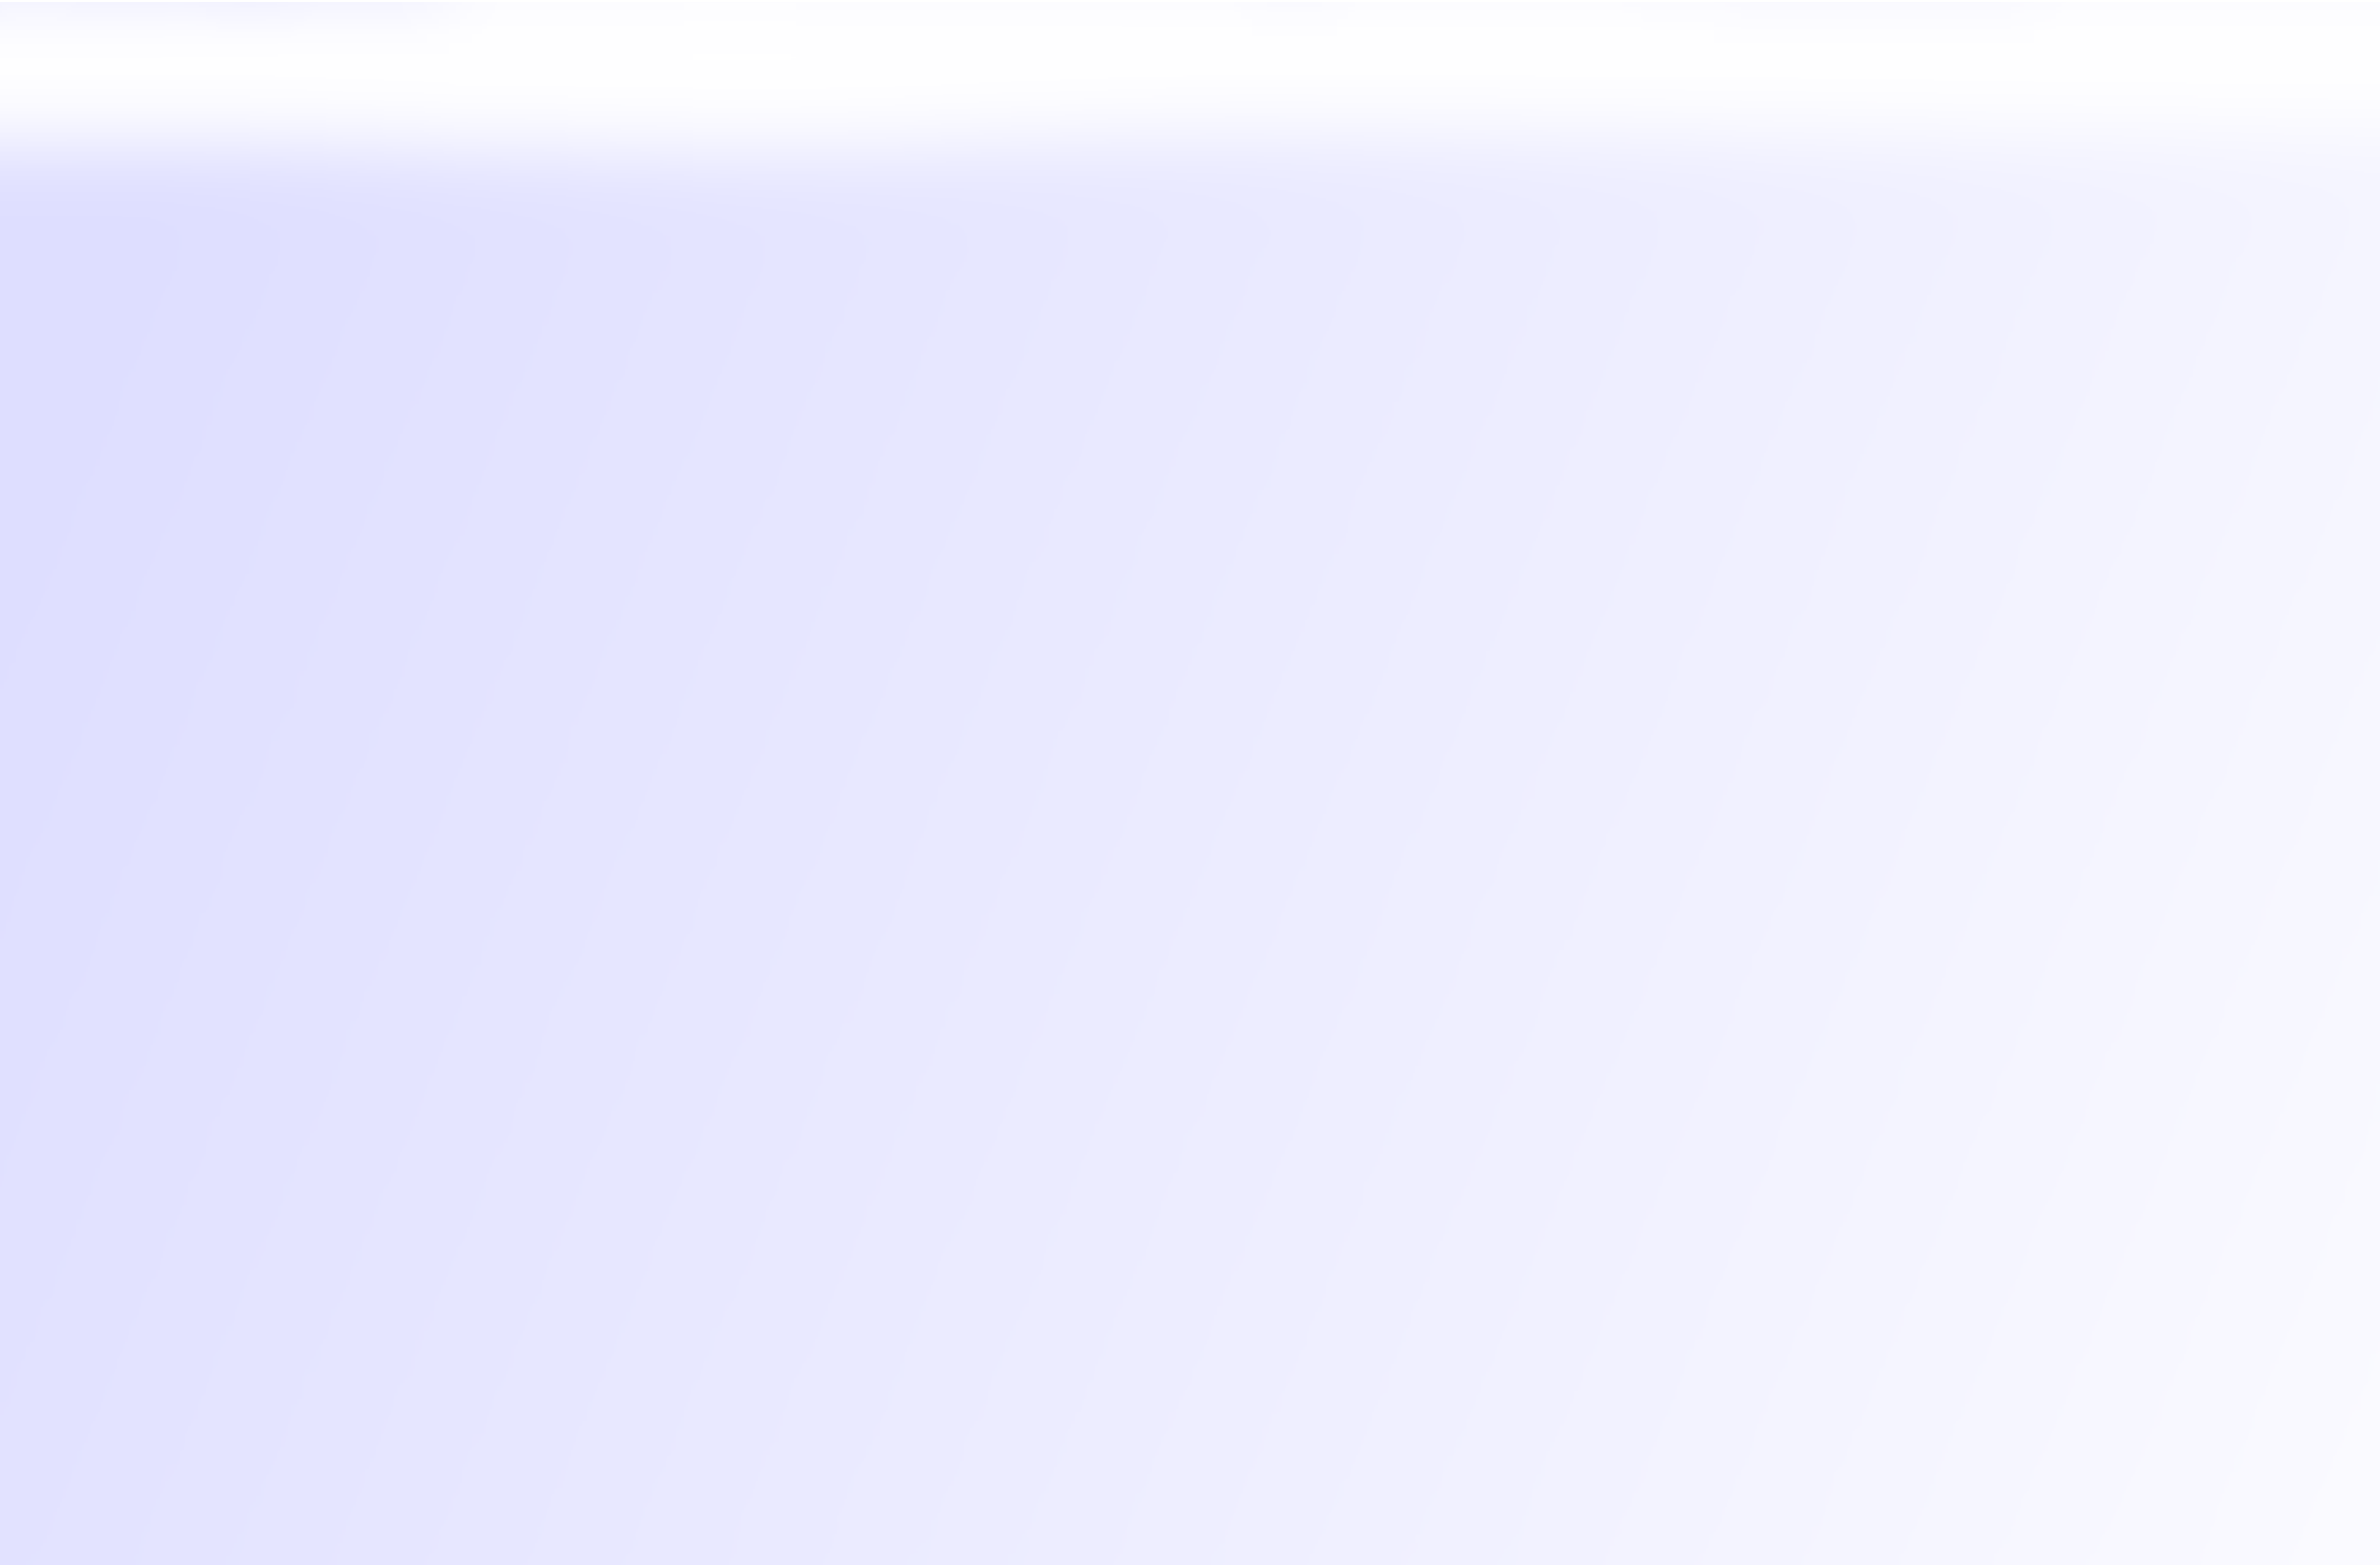
\includegraphics[height=1.1\textheight]{background}};
\end{tikzpicture}
}

\begin{poster}{
grid=false,
borderColor=bordercol, % Border color of content boxes
headerColorOne=headercol1, % Background color for the header in the content boxes (left side)
headerColorTwo=headercol2, % Background color for the header in the content boxes (right side)
headerFontColor=headerfontcol, % Text color for the header text in the content boxes
boxColorOne=boxcolor, % Background color for the content in the content boxes
headershape=roundedright, % Specify the rounded corner in the content box headers
headerfont=\Large\sf\bf, % Font modifiers for the text in the content box headers
textborder=rectangle,
background=user,
headerborder=open, % Change to closed for a line under the content box headers
boxshade=plain
}
{}
%
%----------------------------------------------------------------------------------------
%	TITLE AND AUTHOR NAME
%----------------------------------------------------------------------------------------
%
{\sf\bf \\ Sistema para la detección de faltas basado\\ en redes neuronales artificiales. Caso de aplicación: daños estructurales} % Poster title
{\vspace{0.5em} Jeferson González, Yeiner Arias\\ % Author names
{\smaller jgonzalez@itcr.ac.cr, yarias@itcr.ac.cr}} % Author email addresses
{
\includegraphics[scale=0.6]{logo}} % University/lab logo

%----------------------------------------------------------------------------------------
%	INTRODUCTION
%----------------------------------------------------------------------------------------

\headerbox{Introducción}{name=introduction,column=0,row=0}{
El análisis de vibración es una técnica utilizada para el estudio de los efectos dinámicos en estructuras y la evaluación de posibles daños. Este de ubica dentro de la categoria de ensayos no destructivos, los cual es una aspecto importante en en estructuras de costo elevado y donde los las pruebas destructivos no son una alternativa.

Una red neuronal artificial es un modelo simplificado del sistema neuronal humano. La unidad básica de una red neuronal se llama \textbf{neurona artificial}, cuya función de salida es:

\begin{equation}
\sum_{i=1}^{N} x_i w_{ji} + b
\end{equation}

%\begin{center}
%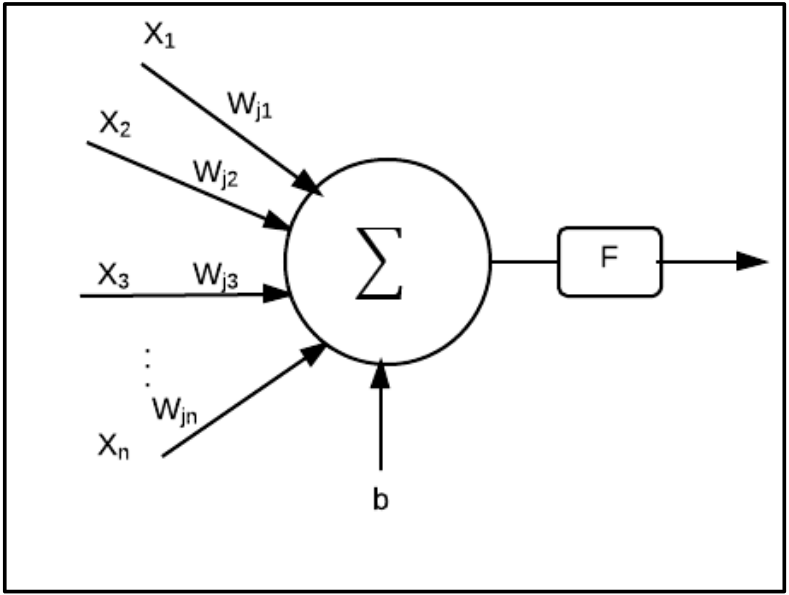
\includegraphics[width=0.49\linewidth]{neurona}
%\\ {\footnotesize \textbf{Figura 1.} Neurona artifical.}
%\end{center}

Con la correcta distribución de capas de neuronas simples, un red neuronal artifical puede utlizarse para diferentes aplicaciones como lo son la identificación de señales/funciones y la \textbf{detección de patrones}. \\

La detección de faltas en sistemas, en general, requiere una distribución de capas y neuronas que les permita \textbf{aprender} el comportamiento del sistema tanto en condiciones normales como en falta. 
\begin{center}
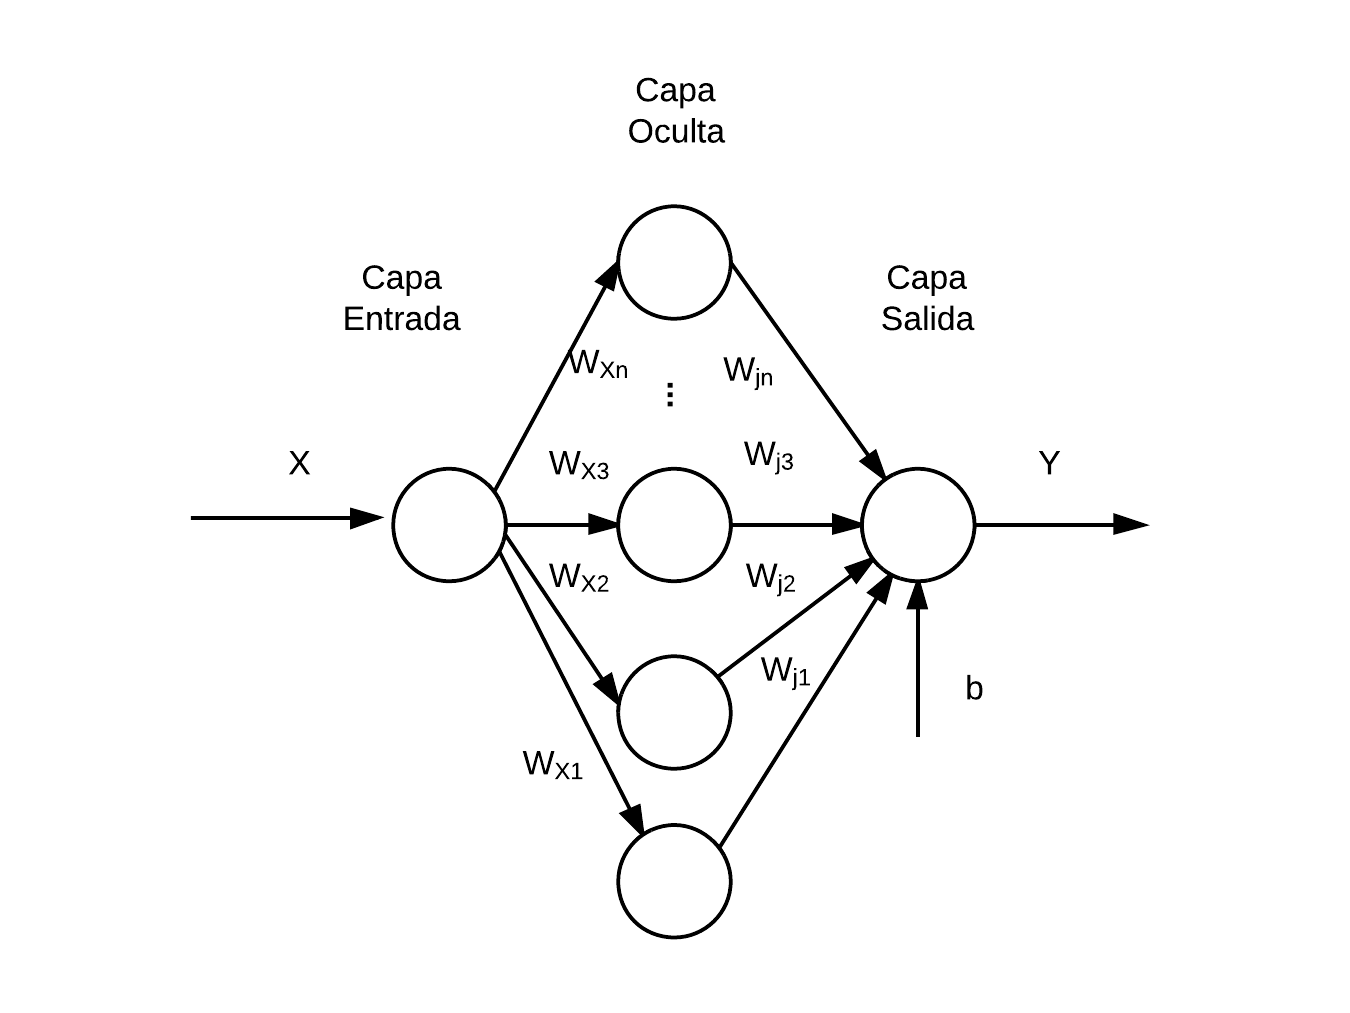
\includegraphics[width=\linewidth]{ann}
\\ {\footnotesize \textbf{Figura 1.} Arquitectura de red con una capa oculta.}
\end{center}

%En este trabajo se utilizó un filtro Butterworth de orden 5 discretizado por el %método de la transformada bilineal para eliminar las frecuencias no deseadas %provenientes de factores externos a la estructura.

corrigiendo cosas

}

%----------------------------------------------------------------------------------------
%	MATERIALS AND METHODS
%----------------------------------------------------------------------------------------

\headerbox{Descripción del experimento}{name=methods,column=0,below=introduction}{

\begin{description}
\item[ER1] Sed a orci non ipsum posuere placerat. Nunc in mi augue, a adipiscing massa. Donec dapibus gravida odio, condimentum convallis urna.
\end{description}
\begin{center}
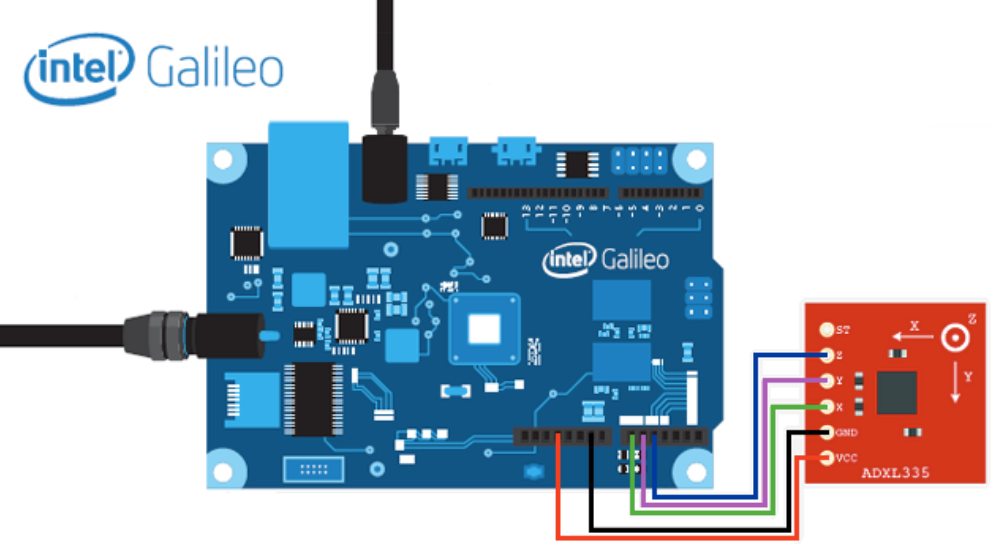
\includegraphics[width=\linewidth]{galileo}
\\ {\footnotesize \textbf{Figura X.} Placa utilizada. Intel Galileo.}
\end{center}

Nullam sollicitudin lobortis urna quis varius. Nullam sagittis blandit diam, $DN = G_t(V_t,E_t)$, risus $E_t \subseteq V_t \times V_t$ ($\forall t \geq 0$). vel tortor justo, $G_0$, quis malesuada lorem.

\begin{equation}
\cos^3 \theta =\frac{1}{4}\cos\theta+\frac{3}{4}\cos 3\theta
\label{eq:refname}
\end{equation}

}

%----------------------------------------------------------------------------------------
%	CONCLUSION
%----------------------------------------------------------------------------------------

\headerbox{Conclusion}{name=conclusion,column=0,below=methods}{

Fusce at erat vitae metus porttitor auctor sit amet at ante. In id dolor tellus, non aliquet elit. Vestibulum bibendum, augue sed laoreet congue, enim nisi ultricies diam, ac pharetra mi dui ut sapien. Maecenas fermentum, neque ut scelerisque consequat, purus leo ultrices nulla, quis scelerisque risus elit non turpis. 

\begin{enumerate}
\item Cras ac ipsum eu nisl imperdiet interdum nunc bibendum, est in pulvinar facilisis, mi purus fringilla tellus, eu varius ipsum ante laoreet ipsum
\item Sed cursus erat quis odio laoreet facilisis maecenas vehicula
\end{enumerate}
}

%----------------------------------------------------------------------------------------
%	REFERENCES
%----------------------------------------------------------------------------------------

\headerbox{References}{name=references,column=0,below=conclusion}{

\smaller % Reduce the font size in this block
\renewcommand{\section}[2]{\vskip 0.05em} % Get rid of the default "References" section title
\nocite{*} % Insert publications even if they are not cited in the poster

\bibliographystyle{unsrt}
\bibliography{sample} % Use sample.bib as the bibliography file
}

%----------------------------------------------------------------------------------------
%	ACKNOWLEDGEMENTS
%----------------------------------------------------------------------------------------

\headerbox{Acknowledgements}{name=acknowledgements,column=0,below=references, above=bottom}{

\smaller % Reduce the font size in this block
Fusce mattis tellus ac odio imperdiet lobortis. Cum sociis natoque penatibus et magnis dis parturient montes, nascetur ridiculus mus. Phasellus commodo blandit euismod. Ut porttitor cursus magna. Mauris adipiscing pellentesque ipsum nec facilisis. Cras ornare bibendum bibendum. Ut a elit purus, vel adipiscing.
} 

%----------------------------------------------------------------------------------------
%	RESULTS 1
%----------------------------------------------------------------------------------------

\headerbox{Transformada discreta de Fourier (DFT)}{name=results1,span=2,column=1,row=0}{ % To reduce this block to 1 column width, remove 'span=2'
Para el caso en estudio, daños en estructuras, las mediciones de vibración en la estructura fueron procesados a través de la Transformada Discreta de Fourier, utilizando la de la biblioteca \textit{FFTW}. 

\begin{center}
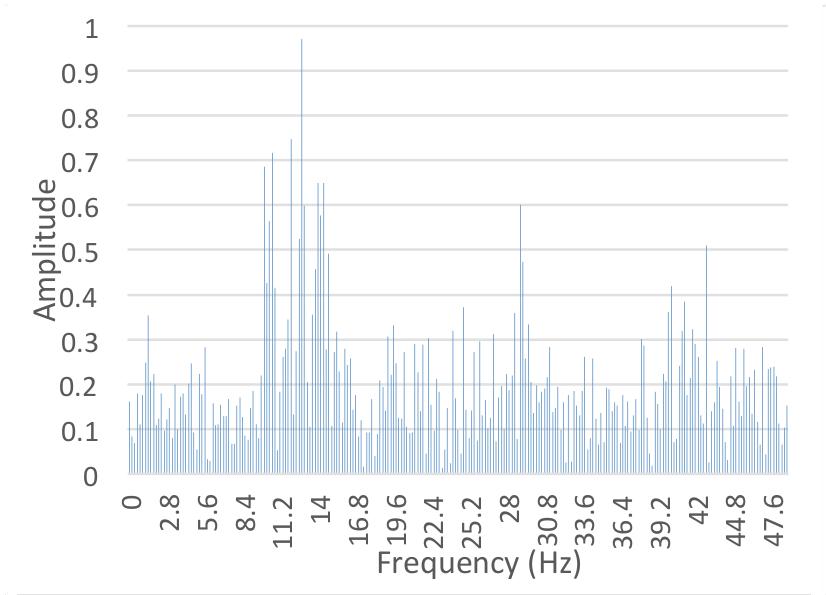
\includegraphics[width=0.5\linewidth]{fft}
\\ {\footnotesize \textbf{Figura X.} DFT de datos de vibración, sin filtrar.}
\end{center}

%------------------------------------------------

%\begin{center}
%\begin{tabular}{l l l}
%\toprule
%\textbf{Treatments} & \textbf{Response 1} & \textbf{Response 2}\\
%\midrule
%Treatment 1 & 0.0003262 & 0.562 \\
%Treatment 2 & 0.0015681 & 0.910 \\
%Treatment 3 & 0.0009271 & 0.296 \\
%\bottomrule
%\end{tabular}
%\captionof{table}{Table caption}
%\end{center}
%}

%----------------------------------------------------------------------------------------
%	RESULTS 2
%----------------------------------------------------------------------------------------

\headerbox{Results Heading 2}{name=results2,span=2,column=1,below=results1,above=bottom}{ % To reduce this block to 1 column width, remove 'span=2'

Nunc sit amet sem ut nulla tincidunt mattis vel nec mauris. Vestibulum odio tellus, lobortis. Vel adipiscing, Aliquam dictum, ligula egestas commodo posuere, lectus lectus congue ligula, sed posuere urna lectus at nisi. Aenean commodo risus ut dolor (viverra scelerisque). Nullam varius, lacus et interdum hendrerit, odio orci ultrices mauris, id interdum eros mauris at urna. Fusce in nisi eros, sit amet volutpat turpis, \textbf{porttior magna} (commodo blandit euismod) \textbf{facilisis ornate magnis} (dis magnis). 

%------------------------------------------------

\begin{center}

\includegraphics[width=0.49\linewidth]{placeholder}

\includegraphics[width=0.49\linewidth]{placeholder}
\captionof{figure}{Figure caption 1 (left); Figure caption 2 (right)}
\end{center}

%------------------------------------------------

Aliquam ac justo lectus. Nunc ultrices aliquet purus non dictum. Nulla facilisi. Quisque vitae urna non purus sollicitudin venenatis. Aliquam erat volutpat. Cum sociis natoque penatibus et magnis dis parturient montes, nascetur ridiculus mus. In hendrerit tortor sed massa consequat eu viverra justo porta. Ut nec felis sem, non elementum.

%------------------------------------------------

<<<<<<< HEAD

=======
ESTO tambien!!
>>>>>>> f6a352198be3a8e1dd64559cba2f6e69adf92762

%------------------------------------------------

Nunc sit amet sem ut nulla tincidunt mattis vel nec mauris. Vestibulum odio tellus, lobortis. Vel adipiscing, Aliquam dictum, ligula egestas commodo posuere, lectus lectus congue ligula, sed posuere urna lectus at nisi. Aenean commodo risus ut dolor (viverra scelerisque). Nullam varius, lacus et interdum hendrerit, odio orci ultrices mauris, id interdum eros mauris at urna. Fusce in nisi eros, sit amet volutpat turpis, \textbf{porttior magna} (commodo blandit euismod) \textbf{facilisis ornate magnis} (dis magnis). Aliquam ac justo lectus. Nunc ultrices aliquet purus non dictum. Nulla facilisi. Quisque vitae urna non purus sollicitudin venenatis. Aliquam erat volutpat. Cum sociis natoque penatibus et magnis dis parturient montes, nascetur ridiculus mus. In hendrerit tortor sed massa consequat eu viverra justo porta. Ut nec felis sem, non elementum.
}

%----------------------------------------------------------------------------------------

\end{poster}

\end{document}